\documentclass[12pt, twoside]{article}
\usepackage[letterpaper, margin=1in, headsep=0.5in]{geometry}
\usepackage[english]{babel}
\usepackage[utf8]{inputenc}
\usepackage{amsmath}
\usepackage{amsfonts}
\usepackage{amssymb}
\usepackage{tikz}
\usetikzlibrary{quotes, angles}
\usepackage{graphicx}
\usepackage{enumitem}
\usepackage{multicol}

\newif\ifmeta
\metatrue %print standards and topics tags

\title{Regents Geometry}
\author{Chris Huson}
\date{September 2020}

\usepackage{fancyhdr}
\pagestyle{fancy}
\fancyhf{}
\renewcommand{\headrulewidth}{0pt} % disable the underline of the header
\raggedbottom


\fancyhead[LE]{\thepage}
\fancyhead[RO]{\thepage \\ Name: \hspace{4cm} \,\\}
\fancyhead[LO]{BECA / Dr. Huson / Geometry 08-Area+volume\\* pset ID: 130}

\begin{document}

\subsubsection*{8-1DN-Circles}
\begin{enumerate}
\item Find the area of $\triangle RAT$. The altitude $h$ of the triangle is 2.7 centimeters and the base $RA=5.4$ cm. Show work by writing an equation before making the calculation.
    \begin{flushright}
    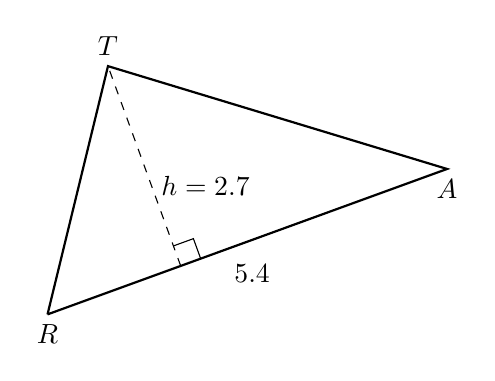
\begin{tikzpicture}[scale=0.9, rotate=20]
      \draw [thick]
        (2,0)node[below]{$R$}--
        (8,0)node[below]{$A$}--
        (4,3)node[above]{$T$} --(2,0);
    \draw [dashed] (4,0)--(4,3);
    \draw (4,0)++(0.3,0)--++(0,0.3)--+(-0.3,0);
    \node at (4,1.2)[right]{$h=2.7$};
    \node at (5,-0.2)[below]{$5.4$};
    \end{tikzpicture}
    \end{flushright} \vspace{1.0cm}

\item Find the area of the parallelogram $ABCD$ shown below, with $AB=40$ millimeters and height $h=24$ mm.
    \begin{flushright}
    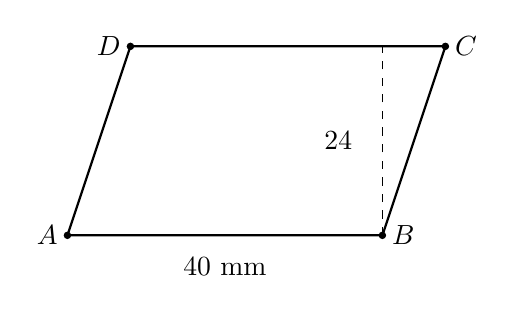
\begin{tikzpicture}[scale=0.8]
      \draw [-, thick] (0,0)--(5,0)--(6,3)--(1,3)--cycle;
      \draw [-, dashed] (5,0)--(5,3);
      \draw [fill] (0,0) circle [radius=0.05] node[left]{$A$};
      \draw [fill] (5,0) circle [radius=0.05] node[right]{$B$};
      \draw [fill] (6,3) circle [radius=0.05] node[right]{$C$};
      \draw [fill] (1,3) circle [radius=0.05] node[left]{$D$};
      \node at (4.3, 1.5){$24$};
      \node at (2.5, -0.5){40 mm};
    \end{tikzpicture}
    \end{flushright} \vspace{1.0cm}

\item  A wooden cutting board is $11 \frac{1}{4}$ inches long, 8 inches wide, and $1 \frac{1}{2}$ inches thick. Find the volume of wood in cubic inches. \hfill (\textbf{diagram not to scale})
    \begin{flushright}
      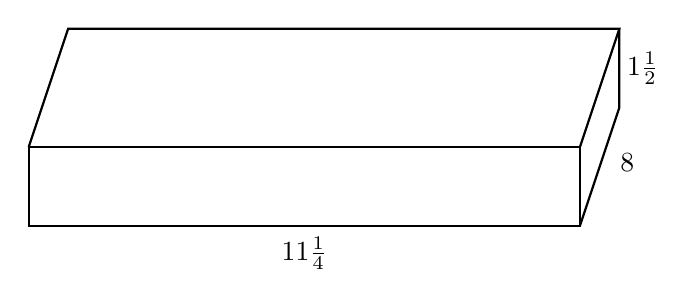
\begin{tikzpicture}[scale=1]
        \draw [-, thick] (0,0)--(7,0)--(7,1)--(0,1)--cycle;
        \draw [-, thick] (0,1)--(0.5,2.5)--(7.5,2.5)--(7,1);
        \draw [-, thick] (7,0)--(7.5,1.5)--(7.5,2.5);
        \node at (7.8, 2){$1 \frac{1}{2}$};
        \node at (3.5, -0.35){$11 \frac{1}{4}$};
        \node at (7.6, 0.8){$8$};
      \end{tikzpicture}
      \end{flushright} \vspace{2cm}

\newpage
\subsubsection*{Model the situation with an equation. Use the formula sheet on the last page. You must start with a labeling variable. \hfill Do NOT solve!}

\item \emph{Worked example:} Find the radius of a circle circumference of 14.7.
\[C=2\pi r=14.7\]

\item A prism has a base area of 20 square centimeters. Its volume is 200 cubic centimeters. Find the prism's height, $h$. \vspace{2cm}

\item A water tank in the shape of a cylinder has a volume of 250 cubic feet. Its height is 12 feet. Find the radius of the base of the tank. \vspace{2cm}

\item A spherical cork fishing net float has a volume of 4000 cubic centimeters. Find its radius. \vspace{2cm}

\item The volume of a cone having a \textbf{diameter} of 10 inches is 200 cubic inches. Find the cone's height. \vspace{2cm}

\item The volume of the Great Pyramid of Giza, the tomb of Pharoah Khufu, is approximately 2,500,000 cubic meters. It is 140 meters tall. Find the area of its base.  \vspace{2cm}

\item The smaller pyramid for his wife, Queen Meretites, has a square base with an area of 2500 square meters. Find the length of the side of its base, $s$.

\newpage
\item In your notebook, write the formulas for the area and circumference of circles:
\[A=\pi r^2\]
\[C=\pi D = 2\pi r\]

\item Given the circle centered at $O$ with radius $r=4$.
  \begin{multicols}{2}
    \begin{enumerate}
      \item Find the circumference of a circle. %\vspace{1cm}
      \item Find the area of the circle.\vspace{3cm}
    \end{enumerate}
    %\columnbreak
    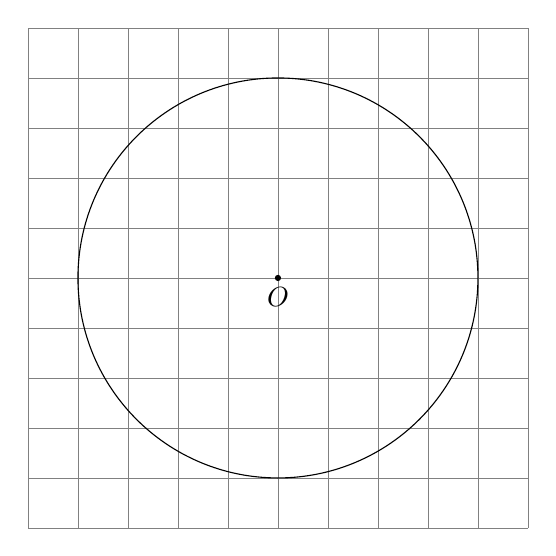
\begin{tikzpicture}[scale=.635]
      \draw [help lines] (-5,-5) grid (5,5);
      %\draw [thick, ->] (-2.2,0) -- (10.4,0) node [below right] {$x$};
      %\draw [thick, ->] (0,-2.2)--(0,10.4) node [left] {$y$};
      \draw (0,0) circle [radius=4] node[below]{$O$};
      \draw [fill] (0,0) circle [radius=0.05];
    \end{tikzpicture}
  \end{multicols}

\item Given the semi-circle shown with diameter $AB=6$. Find its area and perimeter.
    \begin{flushright}
    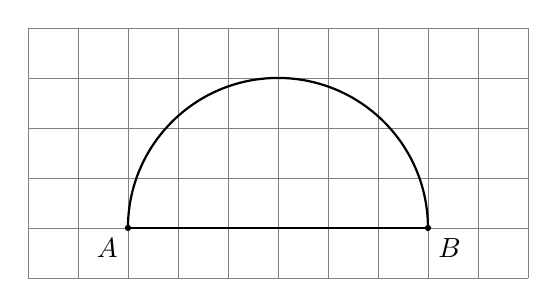
\begin{tikzpicture}[scale=.635]
      \draw [help lines] (-5,-1) grid (5,4);
      \draw [thick] (-3,0)node[below left]{$A$} -- (3,0)node[below right]{$B$};
      %\draw [thick, ->] (0,-2.2)--(0,10.4) node [left] {$y$};
      \draw [thick] (3,0) arc (0:180:3);
      \draw [fill] (-3,0) circle [radius=0.05];
      \draw [fill] (3,0) circle [radius=0.05];
    \end{tikzpicture}
  \end{flushright} \vspace{1cm}

\item Find the radius of a circle having an area of $25 \pi$. \vspace{2cm}
\item Find the diameter of a circle with a circumference of 31.416.

\newpage
\subsubsection*{Equation-of-a-circle algebra competencies} 
  
\item Expand each binomial-squared expression to the form $ax^2+bx+c$.
  \begin{multicols}{2}
  \begin{enumerate}[itemsep=3cm]
    \item $(x+3)(x+3)$
    \item $(x+2)^2$ 
    \item $(x+5)^2$ 
    \item $(x+7)^2$ 
  \end{enumerate}
  \end{multicols}\vspace{3cm}
  
\item Simplify each radical.
  \begin{multicols}{2}
    \begin{enumerate}[itemsep=2cm]
      \item $\sqrt{50}$ 
      \item $\sqrt{18}$
      \item $\sqrt{27}$ 
      \item $\sqrt{24}$ 
    \end{enumerate}
    \end{multicols}\vspace{2cm}
  
\item Solve for the appropriate variable ($h$ and $r$).
    \begin{multicols}{2}
    \begin{enumerate}[itemsep=2cm]
      \item $Area=\frac{1}{2}(14.8)h=62.9$ 
      \item $Area=\pi r^2=483$ 
    \end{enumerate}
    \end{multicols}\vspace{2cm}
    
\newpage
\subsubsection*{Vocabulary study sheet: Circles (tear this sheet off and save it)}

\item \textbf{Internal line segments:} Circle with center at point $P$, as shown.
    \begin{multicols}{2}
      \begin{itemize}
        \item Diameter $\overline{AB}$
        \item Radius $\overline{CP}$
        \item Chord $\overline{DE}$
        \item Central angle $\angle APC$
        \item Arc $\wideparen{AC}$ (with measure $m\wideparen{AC} = 72^\circ$)
      \end{itemize}
    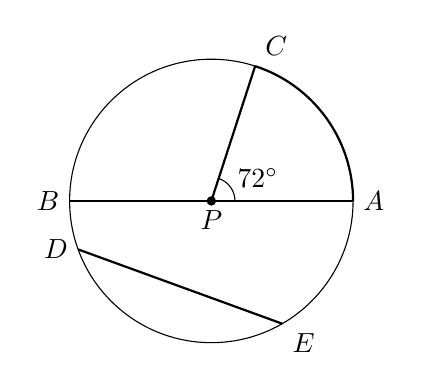
\begin{tikzpicture}[scale=0.6]
      \draw (0,0) circle[radius=3];
      \draw [thick] (3,0) arc (0:72:3);
      \draw [thick] (0:3) node[right] {$A$}--(180:3) node[left] {$B$};
      \draw [thick] (0,0)--(72:3) node[above right] {$C$};
      \draw [thick] (200:3) node[left] {$D$}--(300:3) node[below right] {$E$};
      \fill (0,0) circle[radius=0.1] node[below]{$P$};
      \draw (0.5,0) arc (0:72:0.5) node[right]{$\ 72^\circ$};
      %\draw (35:5) node[right] {$\wideparen{AC}$};
      %\draw (290:5) node[below] {$D$};
    \end{tikzpicture}
  \end{multicols}

\item \textbf{External lines:} Circle with center at point $O$, at right.
    \begin{multicols}{2}
      \begin{itemize}
        \item Secant $\overline{FGH}$
        \item Radius $\overline{OJ}$
        \item Tangent $\overline{FJK}$
        \item Point of tangency $J$
        \item Note: $\overline{OJ} \perp \overline{FJK}$
      \end{itemize}
    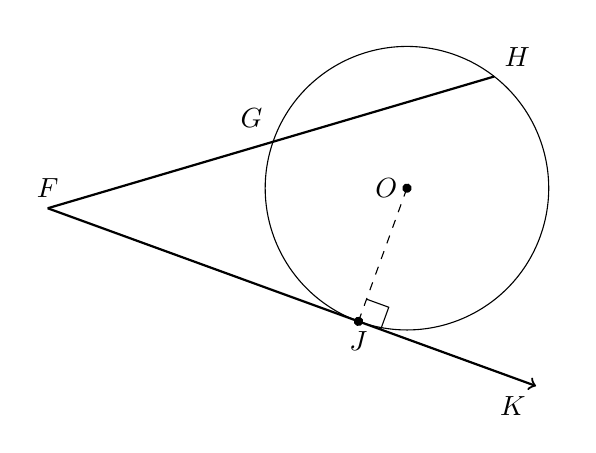
\begin{tikzpicture}[scale=0.6, rotate=-20]
      \draw (0,0) circle[radius=3];
      \draw [thick, ->] (-7,-3) node[above] {$F$}--(4,-3) node[below left] {$K$};
      \draw [thick] (-7,-3)--(72:3) node[above right] {$H$};
      \draw [dashed] (0,-3) node[below] {$J$}--(0,0);
      \fill (0,0) circle[radius=0.1] node[left]{$O$};
      \fill (0,-3) circle[radius=0.1];
      \draw (0,-3) ++(0.5,0)-- ++(0,0.5)--++(-0.5,0);
      \draw (170:3.8) node[below] {$G$};
    \end{tikzpicture}
  \end{multicols}
    
\item \textbf{Areas:} Circle with center at point $Q$.
    \begin{multicols}{2}
      \begin{itemize}
        \item Diameter $\overline{RS}$
        \item Semi-circle $RST$
        \item Sector $QUV$
      \end{itemize}
    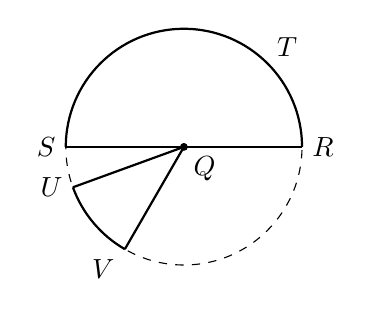
\begin{tikzpicture}[scale=0.5]
      \draw [dashed](0,0) circle[radius=3];
      \draw [thick] (0,0) ++(3,0) arc (0:180:3);
      \draw [thick] (200:3) arc (200:240:3);
      \draw [thick] (0:3) node[right] {$R$}--(180:3) node[left] {$S$};
      \draw [thick] (0,0)--(200:3) node[left] {$U$};
      \draw [thick] (0,0)--(240:3) node[below left] {$V$};
      \fill (0,0) circle[radius=0.1] node[below right]{$Q$};
      \draw (50:3.3) node[right] {$T$};
    \end{tikzpicture}
  \end{multicols}

  \begin{multicols}{2}
\item \textbf{Inscribed polygons and angles:} Circle with triangle inscribed.
      \begin{itemize}
        \item Inscribed $\triangle XYZ$ \vspace{0.5cm}
        \item Inscribed $\angle XYZ$ %\vspace{1cm}
      \end{itemize} \hspace{1cm}
    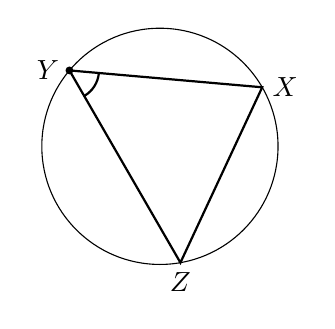
\begin{tikzpicture}[scale=0.5]
      \draw (0,0) circle[radius=3];
      \draw [thick] (140:3) ++(-60:0.75) arc (-60:-5:0.75);
      \draw [thick] (30:3) node[right] {$X$}--(140:3) node[left] {$Y$}
      --(280:3)node[below] {$Z$}--cycle;
      %\draw [thick] (0,0)--(200:3) node[left] {$U$};
      %\draw [thick] (0,0)--(240:3) node[below left] {$V$};
      \fill (140:3) circle[radius=0.1];
      %\draw (50:3.3) node[right] {$T$};
    \end{tikzpicture}
  \end{multicols}

\newpage
\item Triangle vocabulary: vertex, side, hypotenuse, acute, obtuse, perpendicular, median, altitude, perpendicular bisector
  
\item Situations with right triangle hypotenuses as circle radii.

\item Use the tangent function to determine the measure of the central angle $\theta$.
  
\item A regular pentagon is inscribed in a circle as shown below. What is the measure of the central angle between two consecutive vertices, $m\angle AOB$?

\end{enumerate}
\end{document}